\documentclass[11pt,a4paper]{article}

\usepackage{fontspec}
\setmainfont{Latin Modern Roman}
\setmonofont{Latin Modern Mono}
\usepackage[margin=2.5cm]{geometry}
\usepackage[table]{xcolor}
\usepackage{booktabs}
\usepackage{array}
\usepackage{tabularx}
\usepackage{enumitem}
\usepackage{titlesec}
\usepackage{fancyhdr}
\usepackage{setspace}
\usepackage{graphicx}
\usepackage{float}
\usepackage{caption}
\usepackage{listings}
\usepackage[hidelinks]{hyperref}

\definecolor{headrow}{HTML}{EDEDED}

\setstretch{1.12}
\emergencystretch=2em
\setlength{\parskip}{4pt}
\setlength{\parindent}{0pt}
\renewcommand{\arraystretch}{1.25}

\titleformat{\section}{\Large\bfseries}{\thesection}{0.7em}{}
\titleformat{\subsection}{\large\bfseries}{\thesubsection}{0.6em}{}
\titlespacing*{\section}{0pt}{16pt}{6pt}
\titlespacing*{\subsection}{0pt}{10pt}{4pt}

\setlist{itemsep=1pt,topsep=3pt,parsep=1pt}

\newcolumntype{Y}{>{\raggedright\arraybackslash}X}
\newcolumntype{P}[1]{>{\raggedright\arraybackslash}p{#1}}
\newcommand{\hrow}{\rowcolor{headrow}}

\renewcommand{\figurename}{Gambar}
\captionsetup{font=small,labelfont=bf}

\lstset{
  language=Java,
  basicstyle=\ttfamily\footnotesize,
  keywordstyle=\relax,
  commentstyle=\itshape,
  numbers=left,
  numberstyle=\tiny,
  numbersep=6pt,
  frame=single,
  breaklines=true,
  columns=fullflexible,
  keepspaces=true,
  showstringspaces=false,
  tabsize=4
}

\pagestyle{fancy}
\fancyhf{}
\fancyfoot[C]{\small \thepage}
\renewcommand{\headrulewidth}{0pt}

\begin{document}

% ---------------- Judul ----------------
\begin{center}
  {\LARGE\bfseries Laporan Tugas Sesi 8}\\[6pt]
  {\large Unit Testing dengan JUnit 5 pada Class \texttt{OrderPricing}}\\[10pt]
\end{center}

\begin{tabularx}{\textwidth}{@{}P{3.4cm}Y@{}}
  \textbf{Nama}            & Bambang Herlambang (NRP 5803024019) \\
  \textbf{Mata kuliah}     & Software Testing, Universitas Katolik Widya Mandala Surabaya \\
  \textbf{Dosen pengampu}  & Philipus Suryo Subandoro \\
  \textbf{Tanggal}         & 19 Oktober 2026 \\
  \textbf{Repositori}      & \href{https://github.com/Bambang-code/software-testing-sesi8-junit}{\small\texttt{https://github.com/Bambang-code/software-testing-sesi8-junit}} \\
\end{tabularx}
\vspace{4pt}
\hrule

% ---------------- 1 ----------------
\section{Pendahuluan}

\subsection{Latar Belakang dan Tujuan}
Unit testing menguji bagian terkecil kode yang dapat diuji, yaitu method atau class, secara terisolasi. Pada piramida pengujian, unit test berada di dasar karena jumlahnya paling banyak, paling cepat dijalankan, dan paling murah dipelihara. Tugas Sesi 8 meminta pembuatan satu class Java dengan minimal tiga method berlogika bersyarat, lalu pengujiannya dengan JUnit 5. Laporan ini mendokumentasikan rancangan, implementasi, dan hasil eksekusi pengujian tersebut.

\subsection{Ketentuan Tugas dan Pemenuhannya}
\begin{center}
\begin{tabularx}{\textwidth}{@{}P{0.9cm}YY@{}}
\toprule
\hrow \textbf{No} & \textbf{Ketentuan} & \textbf{Pemenuhan} \\
\midrule
1 & Minimal 8 test, termasuk 1 \texttt{@ParameterizedTest} berbasis BVA & 15 method test (26 kasus uji), 2 di antaranya parameterized berbasis BVA \\
2 & Minimal 2 test \texttt{assertThrows} untuk skenario negatif & 4 method test dengan 4 pemanggilan \texttt{assertThrows}, semua memverifikasi pesan exception \\
3 & Penggunaan \texttt{@BeforeEach} dan \texttt{@DisplayName} & \texttt{setUp()} dengan \texttt{@BeforeEach}; semua test memakai \texttt{@DisplayName} \\
4 & Tangkapan layar hasil \texttt{mvn test} yang lulus seluruhnya & Gambar~\ref{fig:mvn}: 26 test lulus, \texttt{BUILD SUCCESS} \\
\bottomrule
\end{tabularx}
\end{center}

% ---------------- 2 ----------------
\section{Class yang Diuji}
Class \texttt{OrderPricing} (paket \texttt{marketplace}) berisi logika harga pesanan pada marketplace UMKM lokal. Tema ini dipilih agar sejalan dengan topik sistem yang dikerjakan pada proyek lintas mata kuliah. Class memiliki tiga method berlogika bersyarat.

\begin{center}
\begin{tabularx}{\textwidth}{@{}P{4.4cm}YP{3.0cm}@{}}
\toprule
\hrow \textbf{Method} & \textbf{Aturan} & \textbf{Input tidak valid} \\
\midrule
\texttt{hitung\allowbreak Total\allowbreak Setelah\allowbreak Diskon\allowbreak (subtotal)} & Subtotal di bawah 100.000: tanpa diskon. Mulai 100.000 sampai di bawah 500.000: diskon 5\%. Mulai 500.000: diskon 10\%. & Subtotal negatif \\
\texttt{hitungOngkir(beratKg, ekspres)} & Sampai 1 kg: Rp10.000. Di atas 1 sampai 5 kg: Rp20.000. Di atas 5 kg: Rp20.000 ditambah Rp5.000 per kg tambahan (dibulatkan ke atas). Ekspres dikenai tarif 1,5 kali. & Berat nol atau negatif \\
\texttt{klasifikasi\allowbreak Pelanggan\allowbreak (jumlahPesanan)} & 0 sampai 4 pesanan: BARU. 5 sampai 19: REGULER. 20 atau lebih: LOYAL. & Jumlah pesanan negatif \\
\bottomrule
\end{tabularx}
\end{center}
Input tidak valid ditolak dengan \texttt{IllegalArgumentException}. Kode lengkap tersedia pada Lampiran A.

% ---------------- 3 ----------------
\section{Rancangan Pengujian}

\subsection{Teknik Penentuan Data Uji}
Data uji ditentukan dengan Equivalence Partitioning (EP) dan Boundary Value Analysis (BVA). EP membagi input menjadi kelompok yang diperlakukan sama oleh program (misalnya subtotal tanpa diskon, diskon 5\%, diskon 10\%, dan tidak valid). BVA kemudian memilih nilai di sekitar batas antar kelompok, yaitu tepat di batas, satu langkah di bawah, dan satu langkah di atas, karena kesalahan pada kondisi seperti \texttt{>} versus \texttt{>=} paling sering muncul di titik tersebut.

\subsection{Nilai Uji dan Hasil yang Diharapkan}
\begin{center}
\begin{tabularx}{\textwidth}{@{}P{3.4cm}P{5.0cm}Y@{}}
\toprule
\hrow \textbf{Method} & \textbf{Nilai uji} & \textbf{Hasil yang diharapkan} \\
\midrule
\texttt{hitung\allowbreak Total\allowbreak Setelah\allowbreak Diskon} & 0; 99.999; 100.000; 100.001; 499.999; 500.000; 500.001 & 0; 99.999; 95.000; 95.000,95; 474.999,05; 450.000; 450.000,90 \\
 & $-1$ & \texttt{IllegalArgumentException} (``Subtotal negatif'') \\
\addlinespace
\texttt{hitungOngkir} & 1 kg; 1,01 kg; 5 kg; 5,1 kg; 7 kg (reguler) & Rp10.000; Rp20.000; Rp20.000; Rp25.000; Rp30.000 \\
 & 1 kg (ekspres) & Rp15.000 \\
 & 0 kg; $-2{,}5$ kg & \texttt{IllegalArgumentException} (``Berat harus lebih dari 0'') \\
\addlinespace
\texttt{klasifikasi\allowbreak Pelanggan} & 0; 4; 5; 19; 20; 21 & BARU; BARU; REGULER; REGULER; LOYAL; LOYAL \\
 & $-1$ & \texttt{IllegalArgumentException} (``Jumlah pesanan negatif'') \\
\bottomrule
\end{tabularx}
\end{center}
Pengujian skenario negatif disertakan pada setiap method, karena test yang hanya melewati jalur sukses memberi rasa aman palsu.

% ---------------- 4 ----------------
\section{Implementasi Test}

\subsection{Anotasi dan Assertion yang Digunakan}
\begin{center}
\begin{tabularx}{\textwidth}{@{}P{4.2cm}Y@{}}
\toprule
\hrow \textbf{Elemen} & \textbf{Penggunaan pada test class} \\
\midrule
\texttt{@Test} & Menandai method sebagai test biasa. \\
\texttt{@BeforeEach} & \texttt{setUp()} membuat objek \texttt{OrderPricing} baru sebelum tiap test (tahap Arrange), sehingga tidak ada keadaan yang terbawa antar test. \\
\texttt{@DisplayName} & Nama test yang mudah dibaca pada laporan, ada di semua test. \\
\texttt{@ParameterizedTest} dan \texttt{@CsvSource} & Satu logika test dijalankan dengan tabel data hasil BVA (7 kasus untuk diskon, 6 kasus untuk klasifikasi). \\
\texttt{assertEquals} & Membandingkan hasil dengan nilai harapan. Untuk tipe \texttt{double} dipakai toleransi (delta) 0,001. \\
\texttt{assertThrows} & Memastikan input tidak valid melempar \texttt{IllegalArgumentException}; semua test exception memverifikasi pesan galat dengan \texttt{assertEquals} pada \texttt{getMessage()}. \\
\bottomrule
\end{tabularx}
\end{center}
Setiap test mengikuti pola Arrange-Act-Assert: objek disiapkan oleh \texttt{setUp()}, method yang diuji dipanggil (Act), lalu hasilnya diperiksa (Assert).

\subsection{Daftar Test}
\begin{center}
\small
\begin{tabularx}{\textwidth}{@{}P{0.8cm}P{5.7cm}YP{1.2cm}@{}}
\toprule
\hrow \textbf{No} & \textbf{Method test} & \textbf{Fokus} & \textbf{Kasus} \\
\midrule
1 & \texttt{tanpaDiskonDiBawahBatas} & Batas: 99.999, tanpa diskon & 1 \\
2 & \texttt{diskonLimaPersenDiBatasBawah} & Batas: 100.000, diskon 5\% & 1 \\
3 & \texttt{diskonSepuluhPersenDiBatasAtas} & Batas: 500.000, diskon 10\% & 1 \\
4 & \texttt{diskonNilaiBatas} & \texttt{@ParameterizedTest} BVA diskon & 7 \\
5 & \texttt{subtotalNegatifDitolak} & Negatif: \texttt{assertThrows} dan pesan galat & 1 \\
6 & \texttt{ongkirTepatDiBatasSatuKilo} & BVA: 1 kg (batas atas tier 1) & 1 \\
7 & \texttt{ongkirTepatDiAtasSatuKilo} & BVA: 1,01 kg (tepat di atas batas tier 1) & 1 \\
8 & \texttt{ongkirTepatDiBatasLimaKilo} & BVA: 5 kg (batas atas tier 2) & 1 \\
9 & \texttt{ongkirTepatDiAtasLimaKilo} & BVA: 5,1 kg (tepat di atas batas tier 2) & 1 \\
10 & \texttt{ongkirTierTigaVerifikasiFormula} & Verifikasi formula tier 3: 7 kg & 1 \\
11 & \texttt{ongkirEkspres} & Tarif ekspres 1,5 kali & 1 \\
12 & \texttt{beratNolDitolak} & Negatif: \texttt{assertThrows} dan pesan galat & 1 \\
13 & \texttt{beratNegatifDitolak} & Negatif: \texttt{assertThrows} dan pesan galat & 1 \\
14 & \texttt{klasifikasiNilaiBatas} & \texttt{@ParameterizedTest} BVA klasifikasi & 6 \\
15 & \texttt{jumlahPesananNegatifDitolak} & Negatif: \texttt{assertThrows} dan pesan galat & 1 \\
\midrule
 & \textbf{Total} & & \textbf{26} \\
\bottomrule
\end{tabularx}
\end{center}
Kode lengkap test class tersedia pada Lampiran B.

% ---------------- 5 ----------------
\section{Hasil Eksekusi}

\subsection{Lingkungan}
\begin{center}
\begin{tabularx}{\textwidth}{@{}P{4.2cm}Y@{}}
\toprule
\hrow \textbf{Komponen} & \textbf{Versi} \\
\midrule
Sistem operasi & Windows 11 (amd64) \\
JDK & Eclipse Temurin 21.0.9 \\
Build tool & Apache Maven 3.10.0 \\
Plugin test & maven-surefire-plugin 3.2.5 \\
Framework test & JUnit Jupiter 5.10.2 (\texttt{junit-jupiter}, mencakup modul \texttt{params}) \\
Editor & Visual Studio Code \\
\bottomrule
\end{tabularx}
\end{center}

\subsection{Hasil mvn test}
Pengujian dijalankan dengan perintah \texttt{mvn test} dari folder proyek yang berisi \texttt{pom.xml}. Hasilnya ditunjukkan pada Gambar~\ref{fig:mvn}.

\begin{figure}[H]
  \centering
  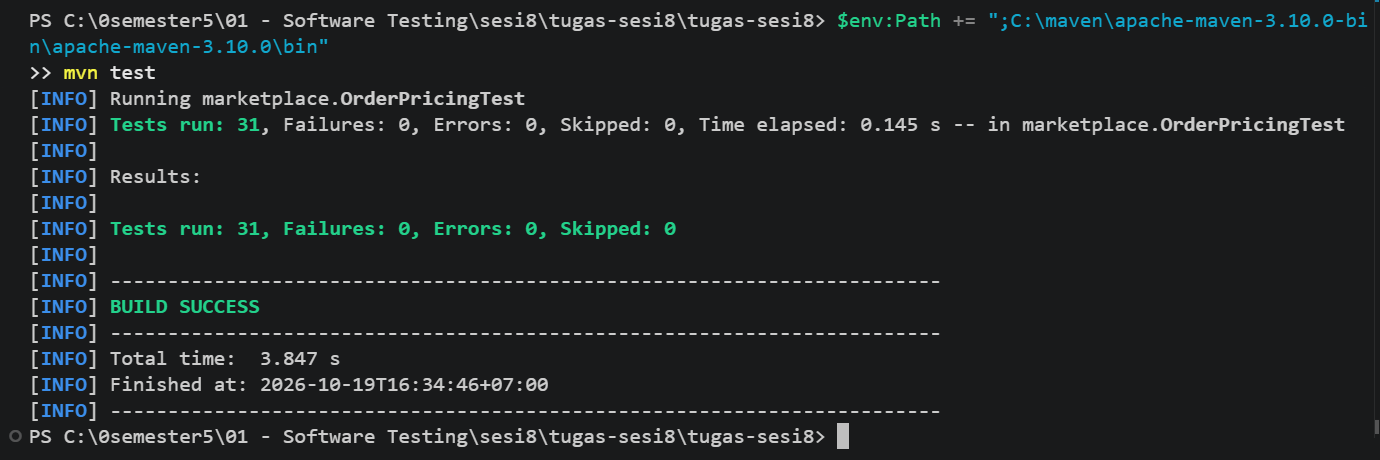
\includegraphics[width=\textwidth]{bukti-terminal.png}
  \caption{Keluaran terminal \texttt{mvn test}: \texttt{Tests run: 26, Failures: 0, Errors: 0, Skipped: 0} dan \texttt{BUILD SUCCESS}.}
  \label{fig:mvn}
\end{figure}

Gambar~\ref{fig:vscode} menampilkan tangkapan layar utuh pada saat yang sama, termasuk struktur proyek (\texttt{src/main}, \texttt{src/test}, \texttt{pom.xml}) dan status editor tanpa galat maupun peringatan (0 error, 0 warning).

\begin{figure}[H]
  \centering
  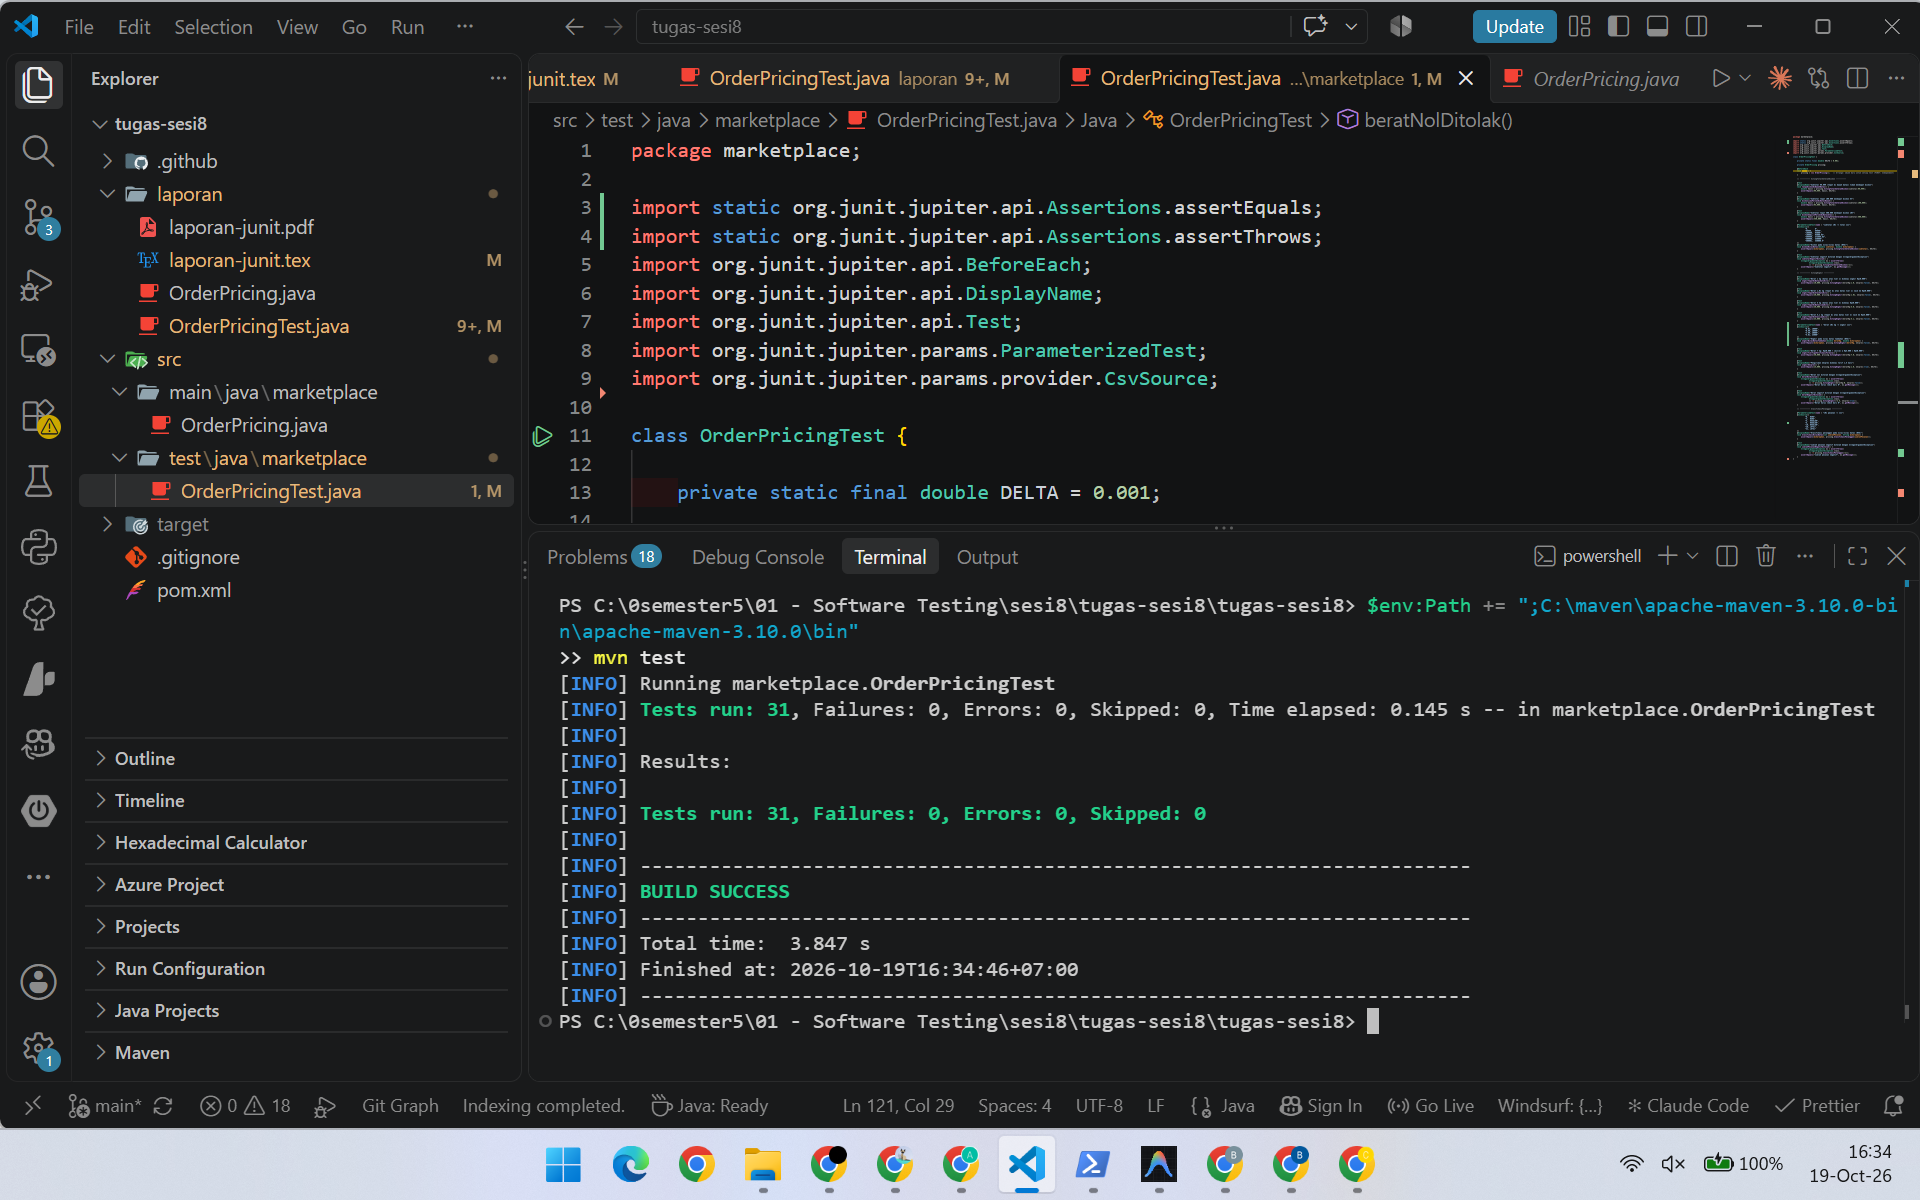
\includegraphics[width=\textwidth]{bukti-mvn-test.png}
  \caption{Tangkapan layar utuh Visual Studio Code setelah \texttt{mvn test} berhasil.}
  \label{fig:vscode}
\end{figure}

\begin{center}
\begin{tabularx}{\textwidth}{@{}P{5.2cm}Y@{}}
\toprule
\hrow \textbf{Indikator} & \textbf{Nilai} \\
\midrule
Tests run & 26 \\
Failures & 0 \\
Errors & 0 \\
Skipped & 0 \\
Waktu eksekusi test & 0,185 detik \\
Status build & BUILD SUCCESS \\
Total waktu build & 3,976 detik \\
Selesai pada & 19 Oktober 2026, 15:26:05 (UTC+7) \\
\bottomrule
\end{tabularx}
\end{center}
Angka 26 berasal dari 13 test biasa ditambah 13 kasus pada dua test parameterized (7 kasus diskon dan 6 kasus klasifikasi). Seluruhnya lulus, dan tidak ada test yang dilewati.

% ---------------- 6 ----------------
\section{Evaluasi terhadap Kriteria Penilaian}

\subsection{Kriteria Tugas}
\begin{center}
\begin{tabularx}{\textwidth}{@{}P{4.1cm}P{1.3cm}Y@{}}
\toprule
\hrow \textbf{Kriteria} & \textbf{Bobot} & \textbf{Bukti pada tugas ini} \\
\midrule
Ketepatan anotasi dan assertion & 30\% & Anotasi siklus hidup, parameterized, dan \texttt{@DisplayName} dipakai sesuai fungsinya; \texttt{assertEquals} memakai delta untuk \texttt{double}, \texttt{assertThrows} untuk exception dengan verifikasi pesan galat pada semua test negatif. \\
Cakupan skenario (batas dan negatif) & 35\% & Nilai batas dari BVA di tiga method (di bawah, tepat, dan di atas batas), serta skenario negatif untuk setiap method. \\
Kualitas penamaan dan kepatuhan FIRST & 20\% & Nama method dan \texttt{@DisplayName} deskriptif; prinsip FIRST dibahas pada subbab berikut. \\
Bukti eksekusi & 15\% & Gambar~\ref{fig:mvn}. \\
\bottomrule
\end{tabularx}
\end{center}

\subsection{Kepatuhan terhadap Prinsip FIRST}
\begin{center}
\begin{tabularx}{\textwidth}{@{}P{3.1cm}Y@{}}
\toprule
\hrow \textbf{Prinsip} & \textbf{Penerapan} \\
\midrule
Fast & Seluruh 26 kasus selesai dalam 0,185 detik karena tidak ada akses database, jaringan, atau berkas. \\
Independent & \texttt{@BeforeEach} membuat objek baru untuk tiap test, tidak ada variabel statis yang berubah, sehingga urutan eksekusi tidak berpengaruh. \\
Repeatable & Tidak bergantung pada waktu, data acak, atau lingkungan eksternal; hasil sama di komputer mana pun. \\
Self-validating & Setiap test memakai assertion sehingga lulus atau gagal otomatis tanpa pemeriksaan manual. \\
Timely & Test ditulis bersamaan dengan class yang diuji, dengan data uji ditentukan dari aturan sebelum eksekusi. \\
\bottomrule
\end{tabularx}
\end{center}

\subsection{Cakupan Cabang dan Keterbatasan}
Penelusuran manual terhadap kode menunjukkan setiap cabang kondisi pada ketiga method dilalui oleh minimal satu test, termasuk cabang ekspres dan non-ekspres serta seluruh cabang validasi. Penelusuran ini bukan pengukuran dengan alat cakupan, karena proyek belum memakai alat seperti JaCoCo. Cakupan yang tinggi juga tidak menjamin tidak ada bug; nilai pengujian terletak pada kebermaknaan assertion dan pemilihan data uji.

% ---------------- 7 ----------------
\section{Kesimpulan}
Class \texttt{OrderPricing} dengan tiga method berlogika bersyarat telah diuji oleh 15 method test (26 kasus uji) memakai JUnit 5. Data uji ditentukan dengan BVA secara konsisten pada semua boundary (batas, tepat di bawah, dan tepat di atas batas) dan dilengkapi skenario negatif untuk tiap method dengan verifikasi pesan exception. Seluruh test lulus pada eksekusi \texttt{mvn test} (26 dijalankan, 0 gagal, 0 error, 0 dilewati), dan rancangan test mengikuti pola Arrange-Act-Assert serta prinsip FIRST. Seluruh ketentuan Tugas Sesi 8 telah terpenuhi.

% ---------------- Lampiran ----------------
\clearpage
\section*{Lampiran A. Kode OrderPricing.java}
\lstinputlisting{OrderPricing.java}

\clearpage
\section*{Lampiran B. Kode OrderPricingTest.java}
\lstinputlisting{OrderPricingTest.java}

% ---------------- Daftar Pustaka ----------------
\section*{Daftar Pustaka}
\begin{enumerate}[label={[\arabic*]},leftmargin=*]
  \item JUnit Team. \textit{JUnit 5 User Guide}. \url{https://junit.org/junit5/docs/current/user-guide}.
  \item Tahchiev, P., et al. \textit{JUnit in Action}. Manning.
  \item Black, R., Graham, D., dan van Veenendaal, E. \textit{Foundations of Software Testing: ISTQB Certification}. Cengage Learning.
  \item Materi kuliah Software Testing, Sesi 8: Unit Testing (Tools: JUnit), Universitas Katolik Widya Mandala Surabaya.
\end{enumerate}

\end{document}
